\documentclass[aspectratio=169]{beamer}

\usepackage[utf8]{inputenc}
\usepackage[T1]{fontenc}
\usepackage{graphicx}
\usepackage{booktabs}
\usepackage{multirow}
\usepackage{amsmath}
\usepackage{tikz}
\usepackage{xcolor}

\usetikzlibrary{positioning, arrows.meta, fit}

\usetheme{Madrid}
\usecolortheme{default}
\setbeamertemplate{navigation symbols}{}
\graphicspath{{images/}}

\title[PrismMathQA]{PrismMathQA: Agentic Math Tutoring with AVSD}
\author{Group 28}
\institute{HUST}
\date{\today}

\newcommand{\tightitems}{
  \setlength{\itemsep}{0.25em}
  \setlength{\parskip}{0pt}
}
\newcommand{\best}[1]{\textbf{#1}}
\newcommand{\second}[1]{\underline{#1}}

\begin{document}

\begin{frame}
  \titlepage
\end{frame}

\begin{frame}{Problem and Goal}
  \small
  \begin{columns}[T,onlytextwidth]
    \begin{column}{0.48\textwidth}
      \begin{block}{Why math tutoring matters}
        \begin{itemize}\tightitems
          \item Correctness matters: fluent explanations are not enough.
          \item Learning requires step-by-step guidance, not just final answers.
          \item Effective tutors adapt to learner context and follow-up questions.
        \end{itemize}
      \end{block}
    \end{column}
    \begin{column}{0.48\textwidth}
      \begin{block}{PrismMathQA goal}
        Build a compact tutor that combines grounded examples, learner memory,
        exact symbolic verification, and a reasoning model trained for
        step-by-step mathematical behavior.
      \end{block}
      \vspace{0.2cm}
      \textbf{Core principle:} the LLM coordinates specialized support instead
      of solving every subproblem alone.
    \end{column}
  \end{columns}
\end{frame}

\begin{frame}{Overall Framework}
  \centering
  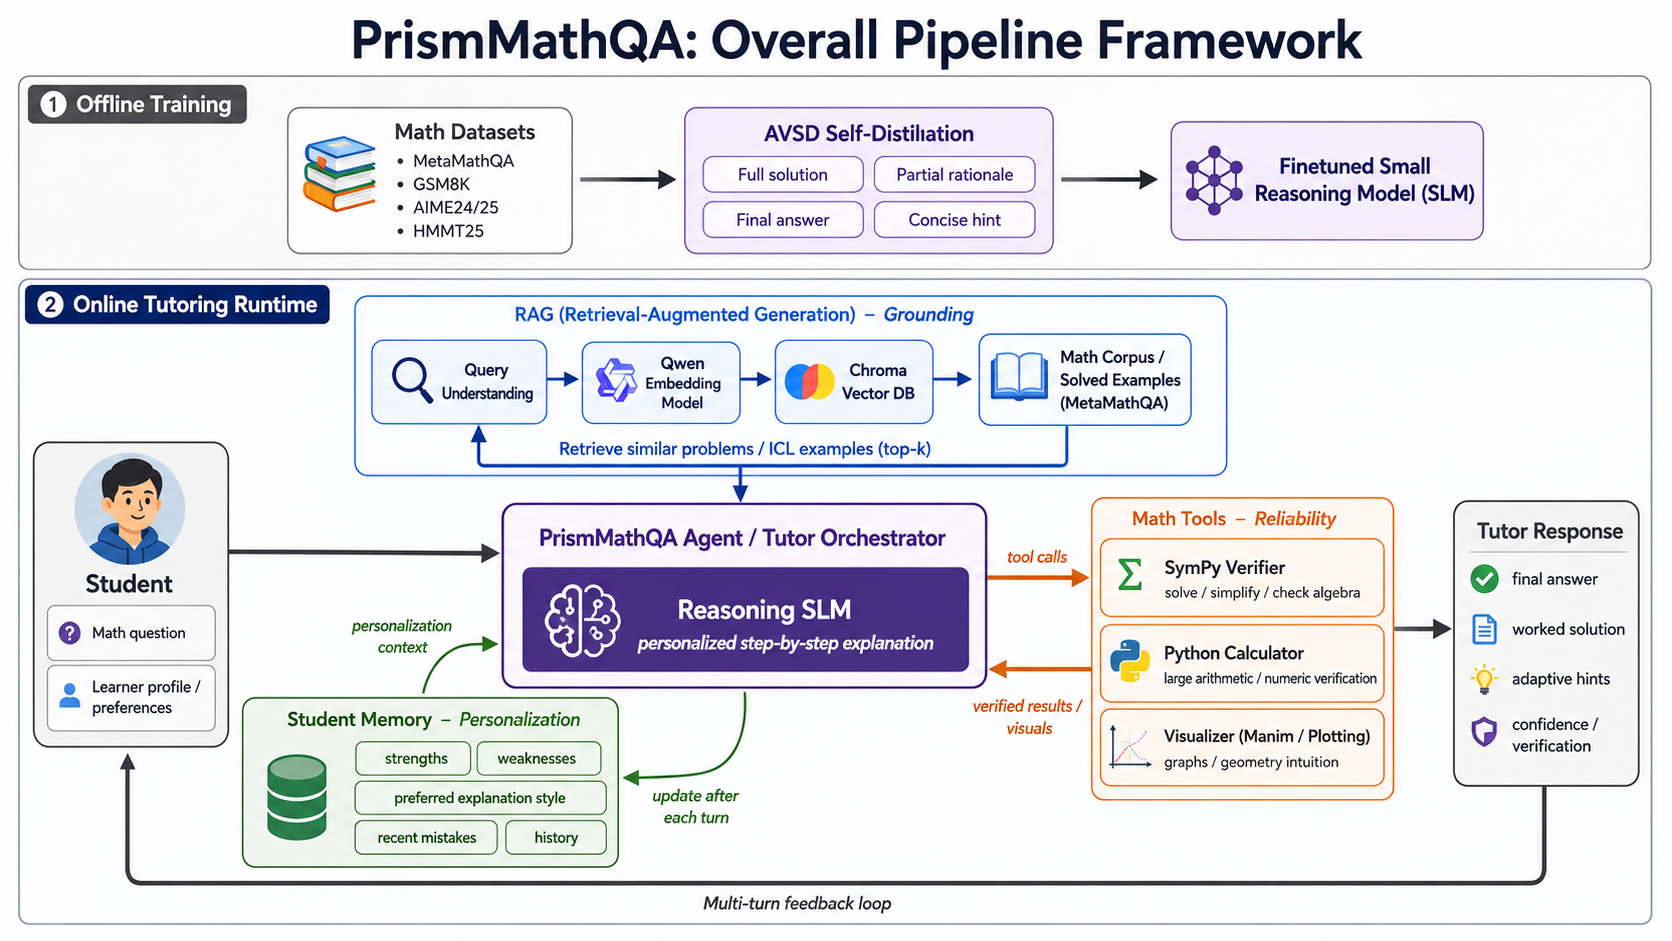
\includegraphics[width=0.96\linewidth,height=0.70\textheight,keepaspectratio]{prism_mathqa_pipeline.png}

  \vspace{0.15cm}
  \small
  \textbf{Offline:} AVSD trains the reasoning model.
  \hspace{0.7cm}
  \textbf{Online:} RAG, memory, and tools support each tutoring turn.
\end{frame}

\begin{frame}{PrismMathQA Pipeline}
  \small
  \begin{center}
  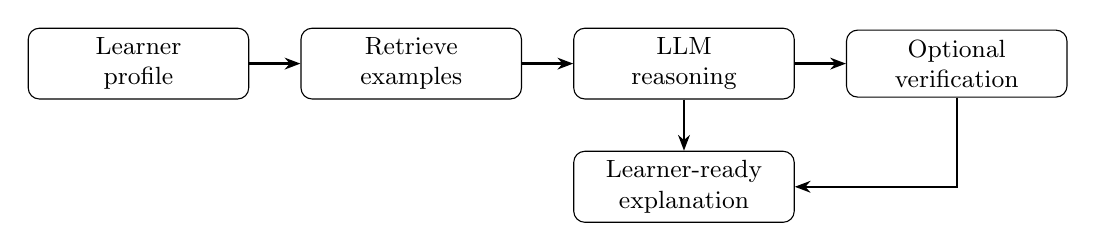
\begin{tikzpicture}[
    node distance=0.65cm,
    box/.style={draw, rounded corners, align=center, minimum width=2.8cm, minimum height=0.85cm, font=\small},
    arr/.style={-{Stealth[length=2mm]}, thick}
  ]
    \node[box] (profile) {Learner\\profile};
    \node[box, right=of profile] (retrieve) {Retrieve\\examples};
    \node[box, right=of retrieve] (reason) {LLM\\reasoning};
    \node[box, right=of reason] (tool) {Optional\\verification};
    \node[box, below=of reason] (answer) {Learner-ready\\explanation};

    \draw[arr] (profile) -- (retrieve);
    \draw[arr] (retrieve) -- (reason);
    \draw[arr] (reason) -- (tool);
    \draw[arr] (tool) |- (answer);
    \draw[arr] (reason) -- (answer);
  \end{tikzpicture}
  \end{center}

  \begin{columns}[T,onlytextwidth]
    \begin{column}{0.48\textwidth}
      \begin{block}{Context}
        Grade level, preferred explanation style, weak areas, and recent
        conversation history guide the response.
      \end{block}
    \end{column}
    \begin{column}{0.48\textwidth}
      \begin{block}{Verification}
        The model asks for a SymPy-backed check when exact computation is
        more trustworthy than free-form generation.
      \end{block}
    \end{column}
  \end{columns}
\end{frame}

\begin{frame}{Agentic Division of Labor}
  \small
  \begin{columns}[T,onlytextwidth]
    \begin{column}{0.48\textwidth}
      \begin{block}{Reasoning LLM}
        Explains the solution, adapts tone and depth, and decides when external
        support is needed. It turns retrieved context and tool outputs into a
        coherent learner-ready explanation.
      \end{block}
      \begin{block}{RAG over MetaMathQA}
        Uses Qwen3-Embedding-0.6B with Chroma to retrieve solved examples that
        expose relevant mathematical patterns and explanation styles. These
        examples ground the response in nearby problems instead of relying only
        on parametric memory.
      \end{block}
    \end{column}
    \begin{column}{0.48\textwidth}
      \begin{block}{Learner memory}
        Stores profile fields, recent interactions, preferences, and weak
        areas for continuity across turns. This lets the tutor adjust pacing
        and avoid treating every question as a fresh session.
      \end{block}
      \begin{block}{SymPy verifier}
        Checks exact arithmetic, algebraic simplification, equation solving,
        and derivatives when reliability matters. The verifier handles
        deterministic computation that free-form generation may get wrong.
      \end{block}
    \end{column}
  \end{columns}
\end{frame}

\begin{frame}{RAG Corpus: MetaMathQA Examples}
  \scriptsize
  \resizebox{\linewidth}{!}{
  \begin{tabular}{p{0.18\linewidth}p{0.31\linewidth}p{0.22\linewidth}p{0.22\linewidth}}
    \toprule
    Question type & Sample problem & Mathematical skill & Why it helps tutoring \\
    \midrule
    Algebraic manipulation &
    Solve $987654321x-123456789=555555555$ as a reduced fraction. &
    Linear equations, exact arithmetic, fraction reduction. &
    Shows clean symbolic transformations and exact intermediate steps. \\
    \midrule
    Coordinate geometry &
    Find the perimeter form $a+b\sqrt{2}+c\sqrt{5}$ for a coordinate hexagon. &
    Distance formula, radicals, geometric modeling. &
    Translates coordinates or diagrams into algebraic quantities. \\
    \midrule
    Functions and graphs &
    For $f(x)=x^2-4x+1$, find the vertex, axis, and minimum value. &
    Completing the square, quadratic interpretation. &
    Connects algebraic manipulation to graph meaning. \\
    \midrule
    Contest reasoning &
    Convert $(x,y)=(2\cos t-\sin t,64\sin t)$ into $ax^2+bxy+cy^2=1$. &
    Parameter elimination, trigonometric substitution. &
    Provides multi-step structure for hard derivations. \\
    \bottomrule
  \end{tabular}}

  \vspace{0.25cm}
  \small
  MetaMathQA is useful because retrieved items include both problem statements
  and worked solution text, so retrieval supplies a reasoning pattern rather
  than just an answer.
\end{frame}

\begin{frame}{Why Fine-tuning Matters}
  \small
  \begin{block}{Runtime support is necessary but not sufficient}
    RAG, memory, and tools improve grounding and reliability, but the base
    model still needs to produce coherent mathematical trajectories before
    external support is applied.
  \end{block}

  \begin{columns}[T,onlytextwidth]
    \begin{column}{0.31\textwidth}
      \begin{block}{SFT}
        Dense traces, but static trajectories may not match the model's own
        rollout distribution.
      \end{block}
    \end{column}
    \begin{column}{0.31\textwidth}
      \begin{block}{RLVR / GRPO}
        Verifiable rewards, but feedback is often sparse and final-answer
        oriented.
      \end{block}
    \end{column}
    \begin{column}{0.31\textwidth}
      \begin{block}{Self-distillation}
        Dense token-level learning signal on the model's own generated
        prefixes.
      \end{block}
    \end{column}
  \end{columns}

  \vspace{0.2cm}
  \textbf{AVSD contribution:} aggregate several privileged teacher views
  without trusting any single view unconditionally.
\end{frame}

\begin{frame}{AVSD Core Idea}
  \centering
  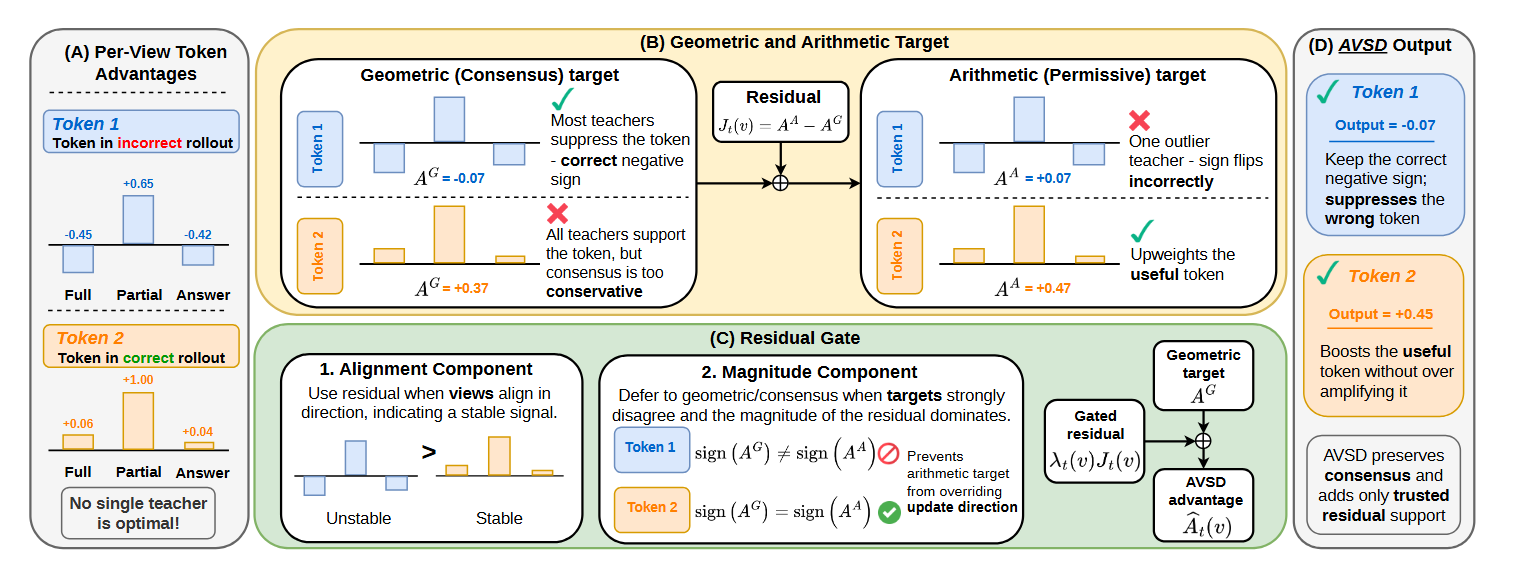
\includegraphics[width=0.98\linewidth,height=0.76\textheight,keepaspectratio]{avsd_pipeline.png}

  \vspace{0.12cm}
  \small
  The student rolls out from the problem only; teacher mode evaluates the same
  prefixes under full solution, partial rationale, final answer, and concise hint.
\end{frame}

\begin{frame}{Preparing Multi-view Data}
  \scriptsize
  \resizebox{\linewidth}{!}{
  \begin{tabular}{p{0.20\linewidth}p{0.36\linewidth}p{0.36\linewidth}}
    \toprule
    View & Teacher context & Training role \\
    \midrule
    Full solution &
    Complete worked derivation with final answer. &
    Provides dense reasoning supervision and exposes the full mathematical structure. \\
    \midrule
    Partial rationale &
    Initial reasoning steps or a truncated rationale. &
    Guides the model toward a useful start without forcing every later step to match a reference. \\
    \midrule
    Final answer &
    Gold answer without the full derivation. &
    Supplies compact correctness information while leaving room for the model's own explanation path. \\
    \midrule
    Concise hint &
    Short hint such as a key substitution, theorem, or transformation. &
    Points toward a productive strategy without revealing the complete solution. \\
    \bottomrule
  \end{tabular}}

  \vspace{0.25cm}
  \small
  These four views are privileged training-time contexts; the deployed student
  model does not receive them at inference time.
\end{frame}

\begin{frame}{Token-level Distillation Signal}
  \small
  \begin{block}{Single-view reverse-KL intuition}
    At prefix $h_t=(x,y_{<t})$, compare the student distribution $p_t$ with a
    privileged teacher distribution $q_t$:
    \[
      A_t(v)=\log q_t(v)-\log p_t(v).
    \]
  \end{block}

  \begin{columns}[T,onlytextwidth]
    \begin{column}{0.48\textwidth}
      \begin{block}{If $A_t(v)>0$}
        The teacher assigns token $v$ higher probability than the student, so
        training promotes that token.
      \end{block}
    \end{column}
    \begin{column}{0.48\textwidth}
      \begin{block}{If $A_t(v)<0$}
        The teacher assigns token $v$ lower probability than the student, so
        training suppresses that token.
      \end{block}
    \end{column}
  \end{columns}

  \vspace{0.2cm}
  Dense token feedback is valuable because many wrong math solutions fail at
  one local algebraic step rather than in the entire trajectory.
\end{frame}

\begin{frame}{Consensus, Residual, and Gate}
  \footnotesize
  \begin{columns}[T,onlytextwidth]
    \begin{column}{0.48\textwidth}
      \begin{block}{Consensus target}
        Geometric mean keeps tokens supported across views:
        \[
          \widetilde{q}_t^G(v)=
          \left(\prod_{m=1}^{M}q_t^{(m)}(v)\right)^{1/M}.
        \]
      \end{block}
      \begin{block}{Arithmetic target and residual}
        Arithmetic mean captures view-specific union support:
        \[
          \begin{aligned}
            q_t^A(v)&=\frac{1}{M}\sum_{m=1}^{M}q_t^{(m)}(v),\\
            J_t(v)&=\log q_t^A(v)-\log \widetilde{q}_t^G(v).
          \end{aligned}
        \]
      \end{block}
    \end{column}
    \begin{column}{0.48\textwidth}
      \begin{block}{Adaptive gate}
        \[
          \widehat{A}_t(v)=A_t^G(v)+\lambda_t(v)J_t(v),
          \quad 0\leq\lambda_t(v)\leq1.
        \]
        The gate admits residual evidence when views align and suppresses it
        when one privileged view dominates.
      \end{block}
      \begin{block}{Reconstructed target}
        \[
          q_t^{\star}(v) \propto
          \widetilde{q}_t^G(v)\exp(\lambda_t(v)J_t(v)).
        \]
      \end{block}
    \end{column}
  \end{columns}
\end{frame}

\begin{frame}{Training Procedure and Lambda Gate}
  \footnotesize
  \begin{columns}[T,onlytextwidth]
    \begin{column}{0.45\textwidth}
      \begin{block}{Training loop}
        \begin{enumerate}\tightitems
          \item Sample a math problem and privileged artifacts from a MetaMathQA subset.
          \item Generate an on-policy rollout from the problem only.
          \item Build four teacher contexts: full, partial rationale, answer, hint.
          \item Evaluate teacher distributions at student prefixes.
          \item Compute $q_t^G$, $q_t^A$, $J_t$, $\lambda_t$, $q_t^\star$.
          \item Minimize reverse-KL to the reconstructed target.
        \end{enumerate}
      \end{block}
    \end{column}
    \begin{column}{0.53\textwidth}
      \begin{block}{Alignment component}
        \[
          C_t(v)=
          \frac{|A_t^G(v)|}
          {\frac{1}{M}\sum_{m=1}^{M}|\Delta_t^{(m)}(v)|+\epsilon}
        \]
        High when teacher views promote or suppress the token in the same direction.
      \end{block}
      \begin{block}{Magnitude component}
        \[
          R_t(v)=\frac{|A_t^G(v)|}{|A_t^G(v)|+J_t(v)+\epsilon},
          \quad
          \lambda_t(v)=C_t(v)R_t(v)
        \]
        Low when residual support is too large relative to consensus.
      \end{block}
    \end{column}
  \end{columns}
\end{frame}

\begin{frame}{Benchmark Analysis: Reported Scores}
  \scriptsize
  \resizebox{\linewidth}{!}{
  \begin{tabular}{p{0.16\linewidth}p{0.27\linewidth}rrrr}
    \toprule
    \multicolumn{2}{c}{Qwen3-4B checkpoint} & \multicolumn{4}{c}{Reported Avg@4} \\
    \cmidrule(lr){1-2}\cmidrule(lr){3-6}
    Method & Training signal & GSM8K & AIME24 & AIME25 & HMMT25 \\
    \midrule
    Base & None & 94.95 & 72.5 & 64.16 & 39.16 \\
    SFT & Static traces & 89.91 & 56.3 & 49.83 & 29.6 \\
    GRPO & Verifiable rewards & 95.81 & 73.14 & 65.70 & 41.82 \\
    OPSD & Single privileged view & 94.98 & 73.31 & 65.46 & 43.31 \\
    RLSD & RLVR + self-distillation & \best{96.89} & \best{77.82} & \second{67.98} & \second{43.59} \\
    AVSD & Multi-context views & \second{96.77} & \second{76.20} & \best{68.29} & \best{44.25} \\
    \bottomrule
  \end{tabular}}

  \vspace{0.25cm}
  \small
  Best results are bolded; second-best results are underlined. RLSD is strongest
  on GSM8K and AIME24, while AVSD is strongest on AIME25 and HMMT25. The table
  keeps the comparison on a fixed Qwen3-4B backbone.
\end{frame}

\begin{frame}{View Ablation Analysis}
  \scriptsize
  \resizebox{0.88\linewidth}{!}{
  \begin{tabular}{lrrrr}
    \toprule
    AVSD view setting & GSM8K & AIME24 & AIME25 & HMMT25 \\
    \midrule
    1 view: full solution & 94.98 & 73.31 & 65.46 & 43.31 \\
    2 views: full + partial rationale & 95.58 & 74.27 & 66.40 & 43.62 \\
    3 views: full + partial rationale + answer & 96.17 & 75.24 & 67.35 & 43.94 \\
    4 views: full + partial rationale + answer + hint & 96.77 & 76.20 & 68.29 & 44.25 \\
    \bottomrule
  \end{tabular}}

  \vspace{0.35cm}
  \small
  \begin{columns}[T,onlytextwidth]
    \begin{column}{0.48\textwidth}
      \begin{block}{Insight 1: More views help}
        Performance rises consistently from 1 to 4 views, showing that the
        teacher family adds useful signal beyond a single full-solution view.
      \end{block}
    \end{column}
    \begin{column}{0.48\textwidth}
      \begin{block}{Insight 2: Harder math benefits}
        The largest gains appear on AIME24 and AIME25, where diverse views help
        stabilize multi-step contest reasoning.
      \end{block}
    \end{column}
  \end{columns}
\end{frame}

\begin{frame}{Demo, Conclusion, and Future Work}
  \centering
  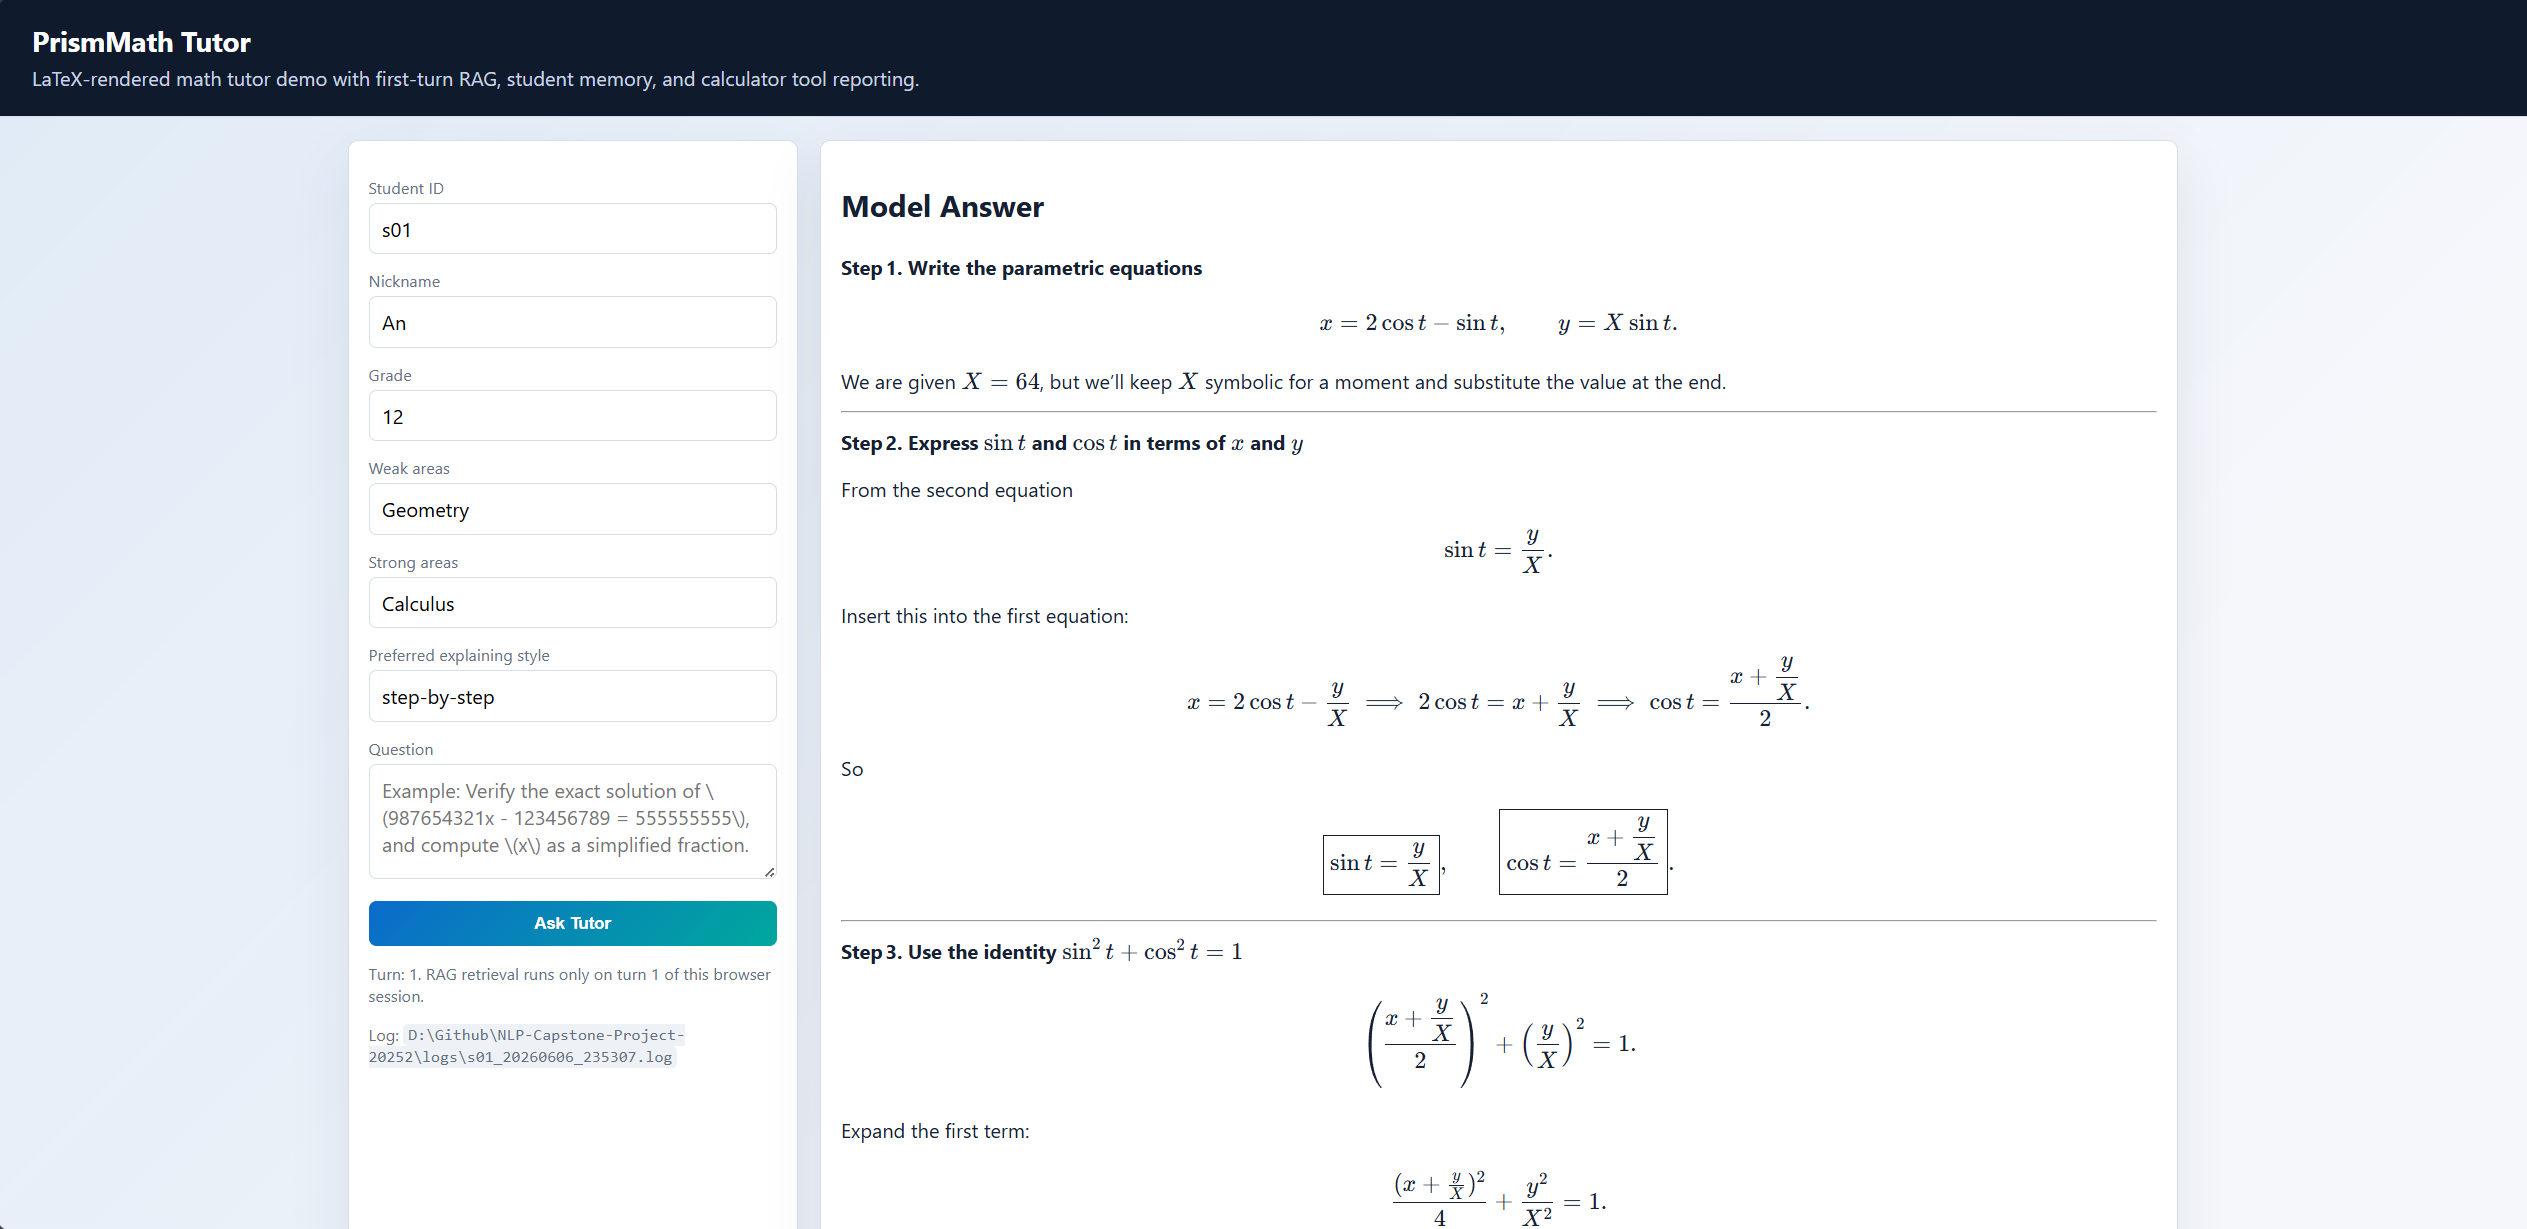
\includegraphics[width=0.98\linewidth,height=0.78\textheight,keepaspectratio]{../nlp_capstone_project/imgs/demo.png}
\end{frame}

\end{document}
